\newpage
\section{Process}

\subsection{Sekvensdiagrammer}
Der er udarbejdet et sekvensdiagram for hver use case. Et sekvensdiagram viser hvordan systemets dele og aktører interagerer med hinanden, og hvilke processer der sker ved disse interaction. Det er beskrevet som sekventiel process og der illustreret diagrammet også hvilke rækkefølge processerne skal eksekveres i. 
Fordi at simplificeret store sekvensdiagrammer gør nogle af dem brug af andre use case, dette ses fx. i sekvensdiagrammet for use case 1. 

\subsection{Konditionering - UC1} \hfil
\begin{figure}[H]
	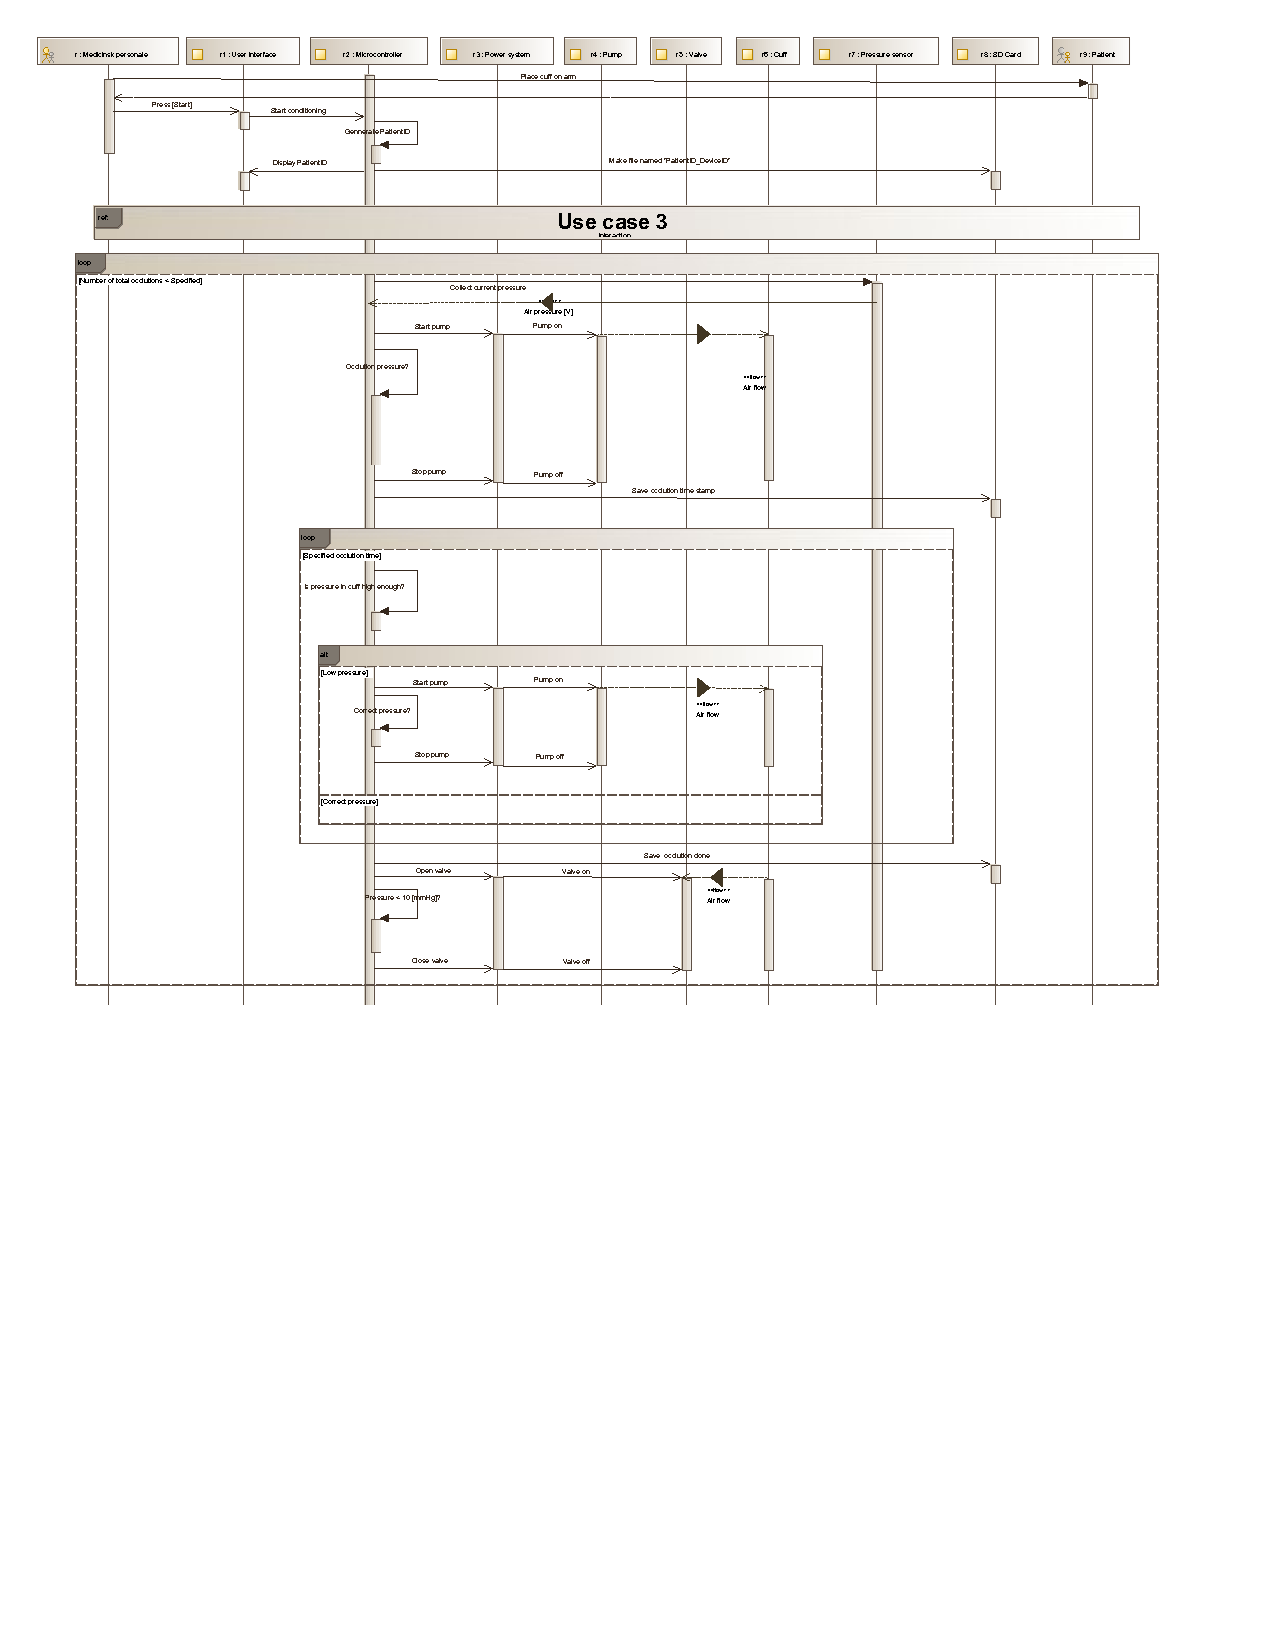
\includegraphics[width=\textwidth ]{pdfs/SD_UC1-crop.pdf}
	\caption{Sekvens diagram over forløb i use case 1}
\end{figure}
\newpage

\subsection{Initialiser blodtryksmåling - UC2}
\begin{figure}[H]
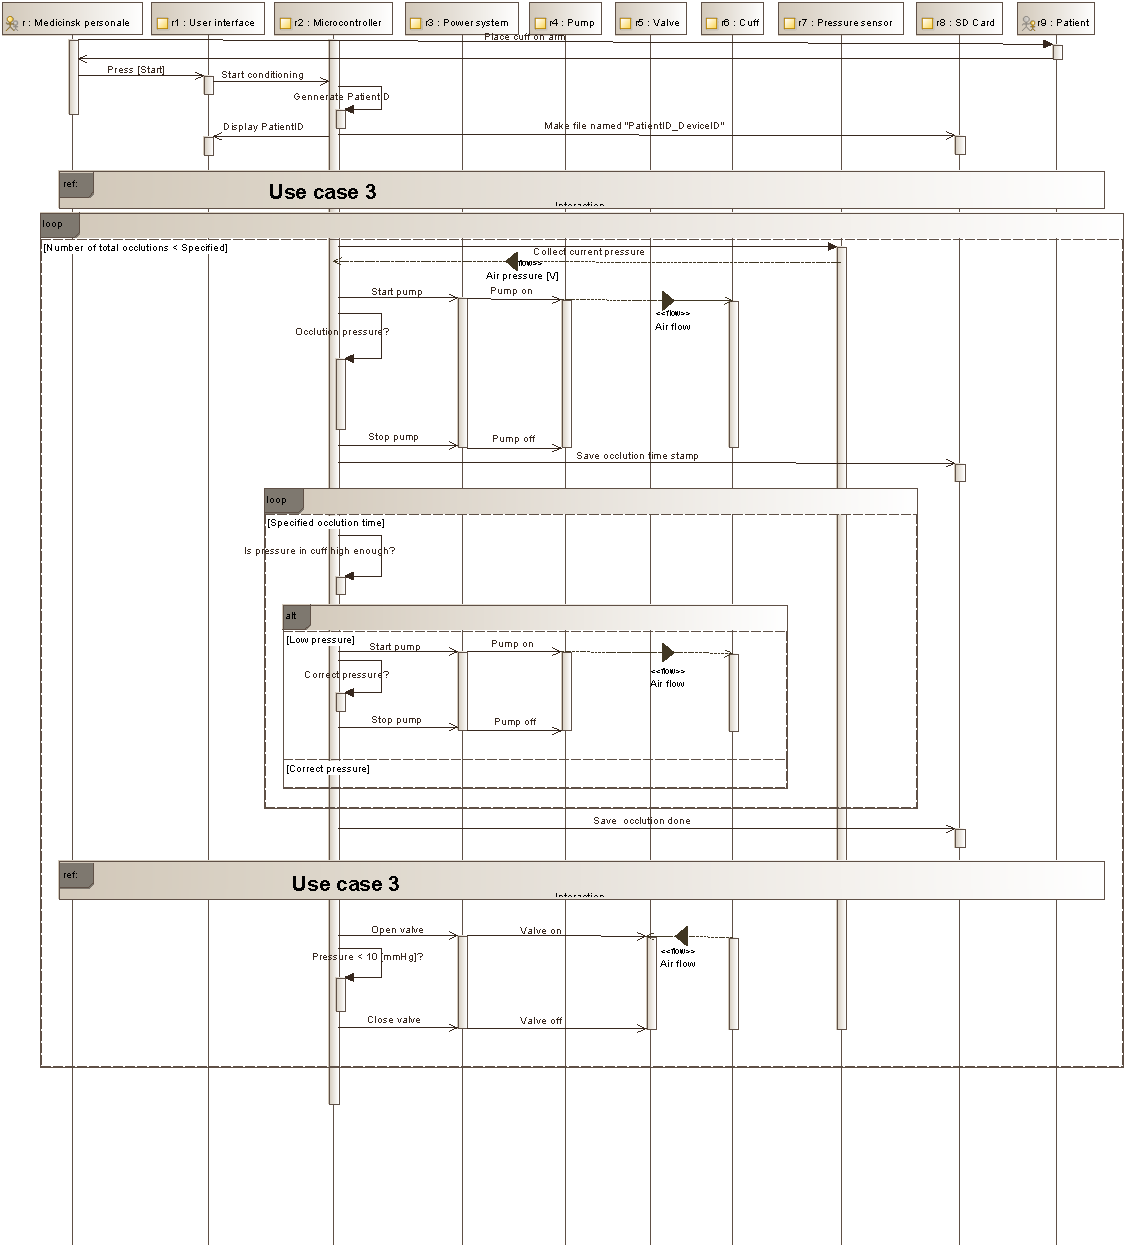
\includegraphics[width=\textwidth]{pdfs/SD_UC2-crop.pdf}
\caption{Sekvens diagram over forløb i use case 2}
\end{figure}
\newpage

\subsection{Mål blodtryk - UC3}
\begin{figure}[H]
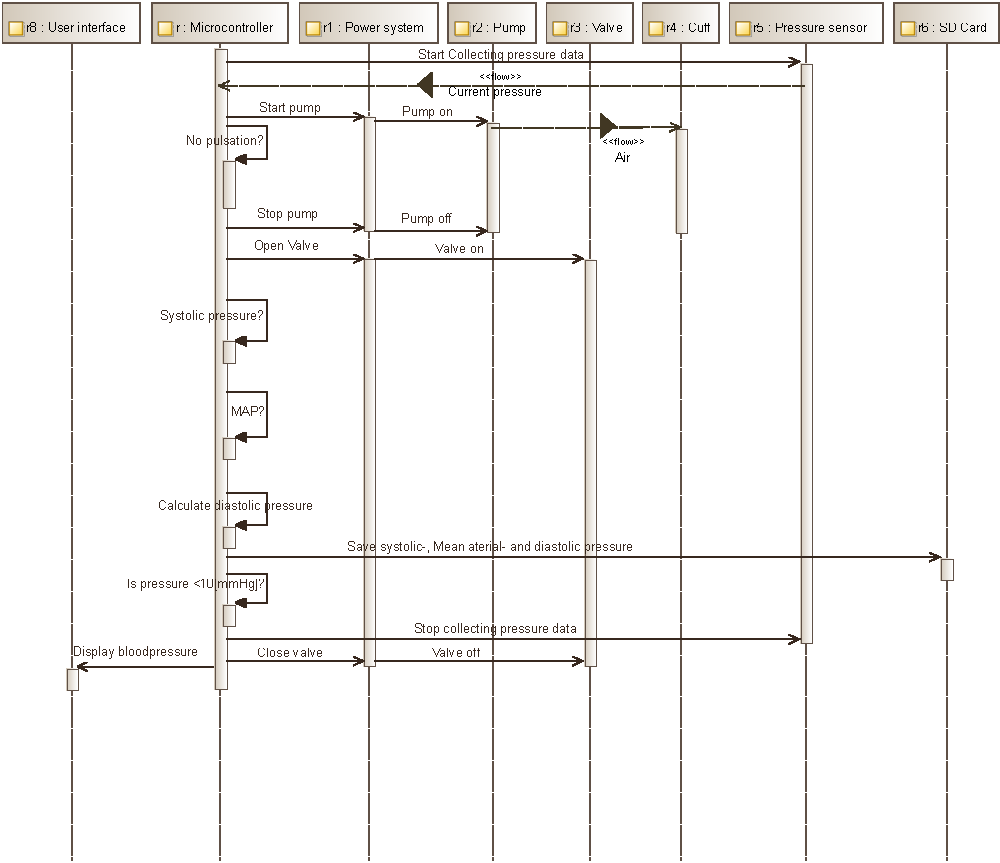
\includegraphics[width=\textwidth]{pdfs/SD_UC3-crop.pdf}
\caption{Sekvens diagram over forløb i use case 3}
\end{figure}
\newpage

\subsection{Overfør data - UC4}
\begin{figure}[H]
\begin{center}
	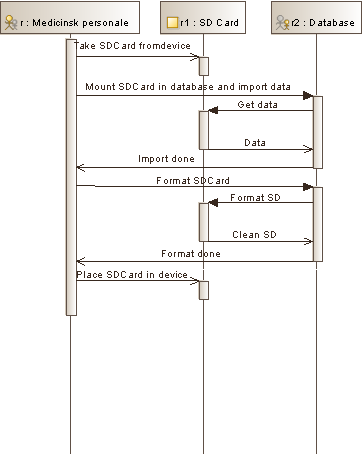
\includegraphics[width=0.60\textwidth]{pdfs/SD_UC4-crop.pdf}
	\caption{Sekvens diagram over forløb i use case 4}
\end{center}
\end{figure}

\newpage

\subsection{Sikkerhedskontrol med pulsoximeter - UC5}
Mangler stadig...

\subsection{Okklusionstræning - UC6}
\begin{figure}[H]
	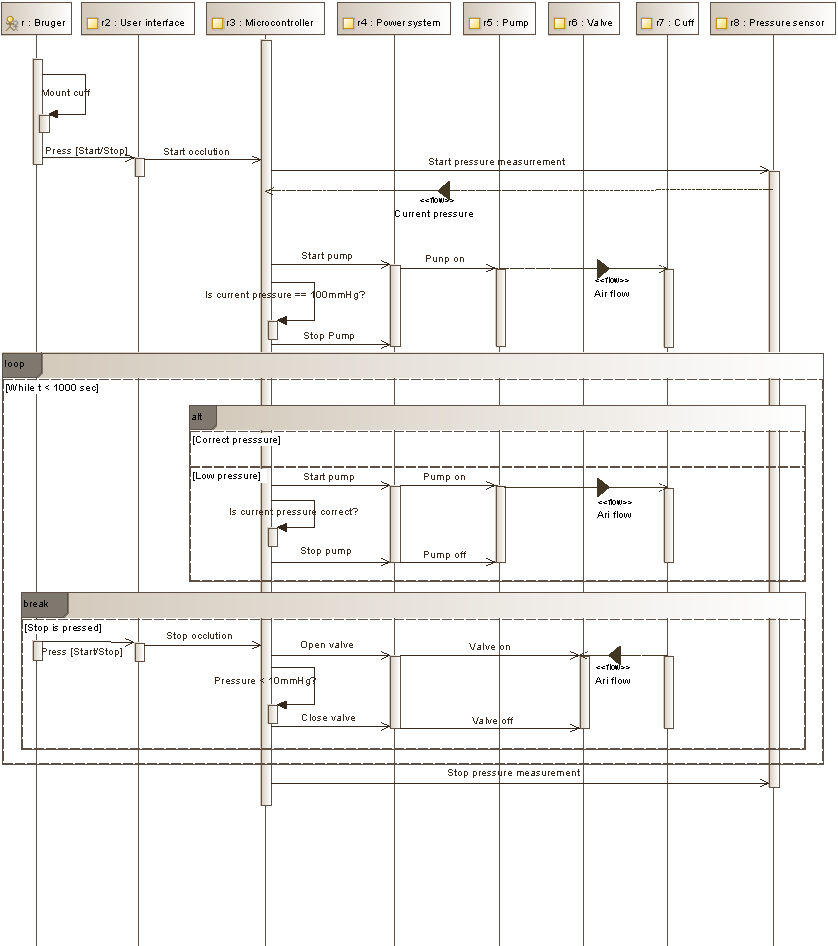
\includegraphics[width=\textwidth]{pdfs/SD_UC6-crop.pdf}
\caption{Sekvens diagram over forløb i use case 6}
\end{figure}
\newpage

\subsection{Afbryd - UC7}
\begin{figure}[H]
	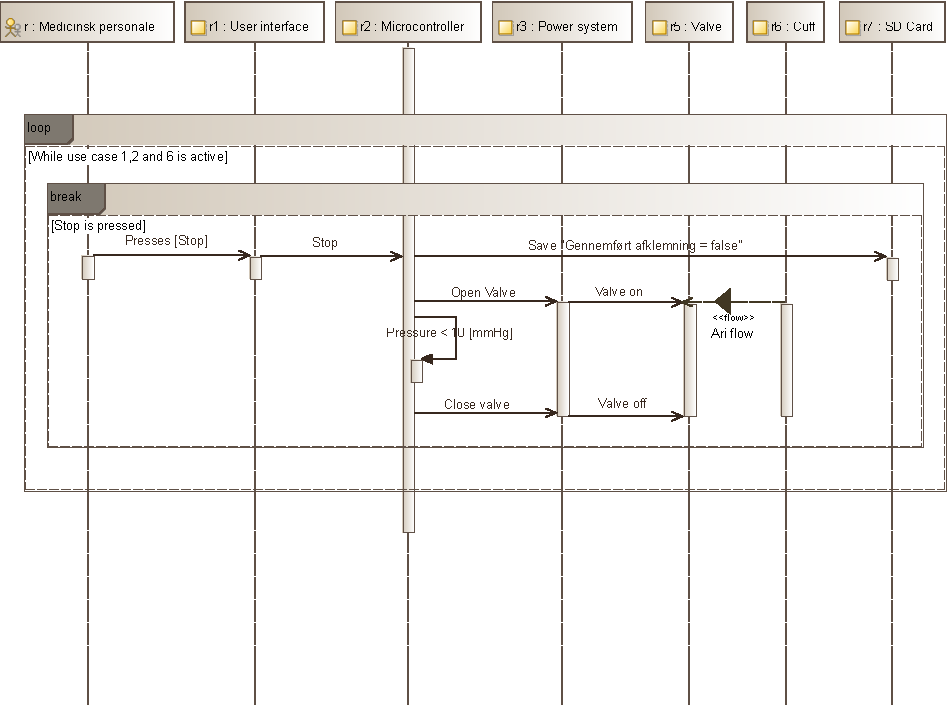
\includegraphics[width=\textwidth]{pdfs/SD_UC7-crop.pdf}
\caption{Sekvens diagram over forløb i use case 7}
\end{figure}
\newpage

\subsection{Setup - UC8}
\begin{figure}[H]
	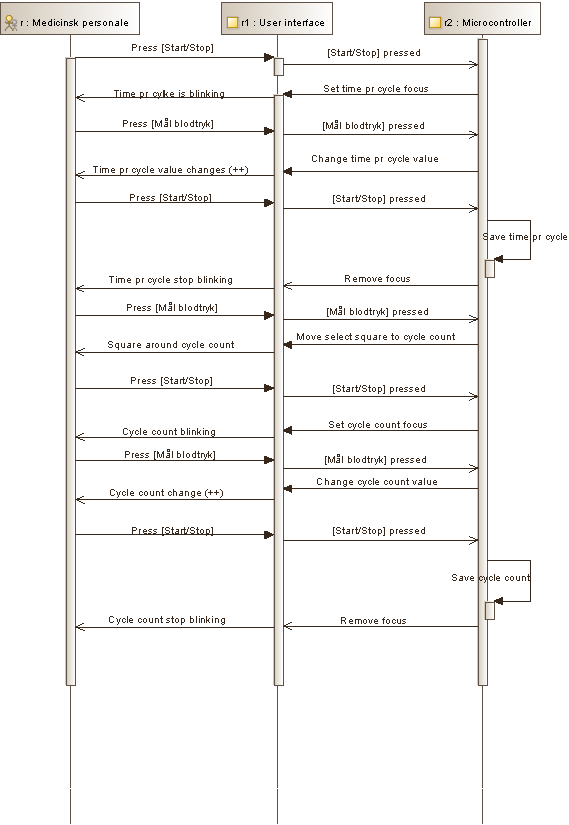
\includegraphics[width=\textwidth]{pdfs/SD_UC8-crop.pdf}
\caption{Sekvens diagram over forløb i use case 8}
\end{figure}
\newpage
